\vskip 0.60cm
\subsection{Introduction}
\vskip 0.25cm
\noindent
Pour la conception et l'implémentation de l'application, nous avons utilisé Visual Studio Code comme Environnement de développement. Nous avons utilisé le framework Flask pour le développement web, sqlite3 pour la base de données nous avons réalisé les algorithmes de traitement en Python. Nous avons aussi d'autres langages tels que JavaScript, HTML, CSS.
\vskip 0.25cm
\subsection{Base de données}
\vskip 0.25cm
\subsubsection{Modèle relationnel}
Voici le modèle relationnel de la base de données utilisée dans notre application :
\newline
\newline
\textbf{Exemple} : une table
\newline
\underline{   } : clé primaire
\newline
\# : clé étrangère
\newline
\newline
\textbf{Candidate}(\underline{id}, firstName, lastName, picture, catchphrase, \#listId, mail, job, identifier, password)
\newline
\textbf{List}(\underline{id}, name, program, politicalEdge)
\newline
\textbf{ProgramGrade}(\underline{id}, \#listId, environment, social, economy)
\newline
\textbf{Users\textunderscore vote}(\underline{id}, \#listId, userIP, economyVote, ecologyVote, socialVote)
\newline
\textbf{Member}(\underline{id}, firstName, lastName, \#listId, job)
\newline
\textbf{jobMemberGrade}(\underline{id}, \#listId, agriexp, artcomchef, cadreprofintsup, profintermed, employe, ouvrier, retraite, sansactprof)
\newline
\textbf{Vote\textunderscore office}(\underline{id}, lat, lon, name)

\subsubsection{Schémas relationnels et contraintes}
Voici le schéma relationnel de la base de donnée utilisé dans notre application :
\newline\newline

\noindent
CREATE TABLE Candidate
    \newline\indent\indent
    (
        \newline\indent\indent\indent
        id INTEGER PRIMARY KEY AUTOINCREMENT,
        \newline\indent\indent\indent
        firstName TEXT,
        \newline\indent\indent\indent
        lastName TEXT,
        \newline\indent\indent\indent
        picture TEXT,
        \newline\indent\indent\indent
        catchphrase TEXT,
        \newline\indent\indent\indent
        listId INTEGER,
        \newline\indent\indent\indent
        email TEXT UNIQUE,
        \newline\indent\indent\indent
        job TEXT,
        \newline\indent\indent\indent
        identifier TEXT UNIQUE,
        \newline\indent\indent\indent
        password TEXT,
        \newline\indent\indent\indent
        FOREIGN KEY (listId) REFERENCES List(id)
    \newline\indent\indent
    );
\newline\newline
CREATE TABLE List
    \newline\indent\indent
    (
        \newline\indent\indent\indent
        id INTEGER PRIMARY KEY AUTOINCREMENT,
        \newline\indent\indent\indent
        name TEXT,
        \newline\indent\indent\indent
        program TEXT,
        \newline\indent\indent\indent
        politicalEdge TEXT
    \newline\indent\indent
    );
\newline\newline
\newpage

CREATE TABLE ProgramGrade
    \newline\indent\indent
    (
        \newline\indent\indent\indent
        id INTEGER PRIMARY KEY AUTOINCREMENT,
        \newline\indent\indent\indent
        listId INTEGER,
        \newline\indent\indent\indent
        environment FLOAT,
        \newline\indent\indent\indent
        social FLOAT,
        \newline\indent\indent\indent
        economy FLOAT,
        \newline\indent\indent\indent
        FOREIGN KEY (listId) REFERENCES List(id)
    \newline\indent\indent
    );
\newline\newline
CREATE TABLE Member
    \newline
    \indent\indent
    (
        \newline
        \indent\indent\indent
        id INTEGER PRIMARY KEY AUTOINCREMENT,
        \newline
        \indent\indent\indent
        firstName TEXT,
        \newline
        \indent\indent\indent
        lastName TEXT,
        \newline
        \indent\indent\indent
        listId INTEGER,
        \newline
        \indent\indent\indent
        job TEXT,
        \newline
        \indent\indent\indent
        FOREIGN KEY (listId) REFERENCES List(id)
    \newline
    \indent\indent
    );
\newline\newline
CREATE TABLE Users\textunderscore vote
    \newline\indent\indent
    (
        \newline\indent\indent\indent
        id INTEGER PRIMARY KEY AUTOINCREMENT,
        \newline\indent\indent\indent
        listId INTEGER,
        \newline\indent\indent\indent
        userIP TEXT NOT NULL,
        \newline\indent\indent\indent
        economyVote INTEGER DEFAULT 0,
        \newline\indent\indent\indent
        ecologyVote INTEGER DEFAULT 0,
        \newline\indent\indent\indent
        socialVote INTEGER DEFAULT 0,
        \newline\indent\indent\indent
        FOREIGN KEY (listId) REFERENCES List(id)
    \newline\indent\indent
    );
\newline\newline
CREATE TABLE Vote\textunderscore office
    \newline\indent\indent
    (
        \newline\indent\indent\indent
        id INTEGER PRIMARY KEY AUTOINCREMENT,
        \newline\indent\indent\indent
        lat FLOAT NOT NULL,
        \newline\indent\indent\indent
        lon FLOAT NOT NULL,
        \newline\indent\indent\indent
        name TEXT NOT NULL
    \newline\indent\indent
    );
\newline\newline
CREATE TABLE jobMemberGrade
    \newline\indent\indent
    (
        \newline\indent\indent\indent
        id INTEGER PRIMARY KEY AUTOINCREMENT,
        \newline\indent\indent\indent
        listId INTEGER NOT NULL,
        \newline\indent\indent\indent
        agriexp INTEGER DEFAULT 0,
        \newline\indent\indent\indent
        artcomchef INTEGER DEFAULT 0,
        \newline\indent\indent\indent
        cadreprofintsup INTEGER DEFAULT 0,
        \newline\indent\indent\indent
        profintermed INTEGER DEFAULT 0,
        \newline\indent\indent\indent
        employe INTEGER DEFAULT 0,
        \newline\indent\indent\indent
        ouvrier INTEGER DEFAULT 0,
        \newline\indent\indent\indent
        retraite INTEGER DEFAULT 0,
        \newline\indent\indent\indent
        sansactprof INTEGER DEFAULT 0,
        \newline\indent\indent\indent
        FOREIGN KEY (listId) REFERENCES List(id)
    \newline\indent\indent
    );
\newline\newline
Pour le schema de la base de donnée voir figure \ref{fig:schemaBD}
\begin{figure}
    \centering
    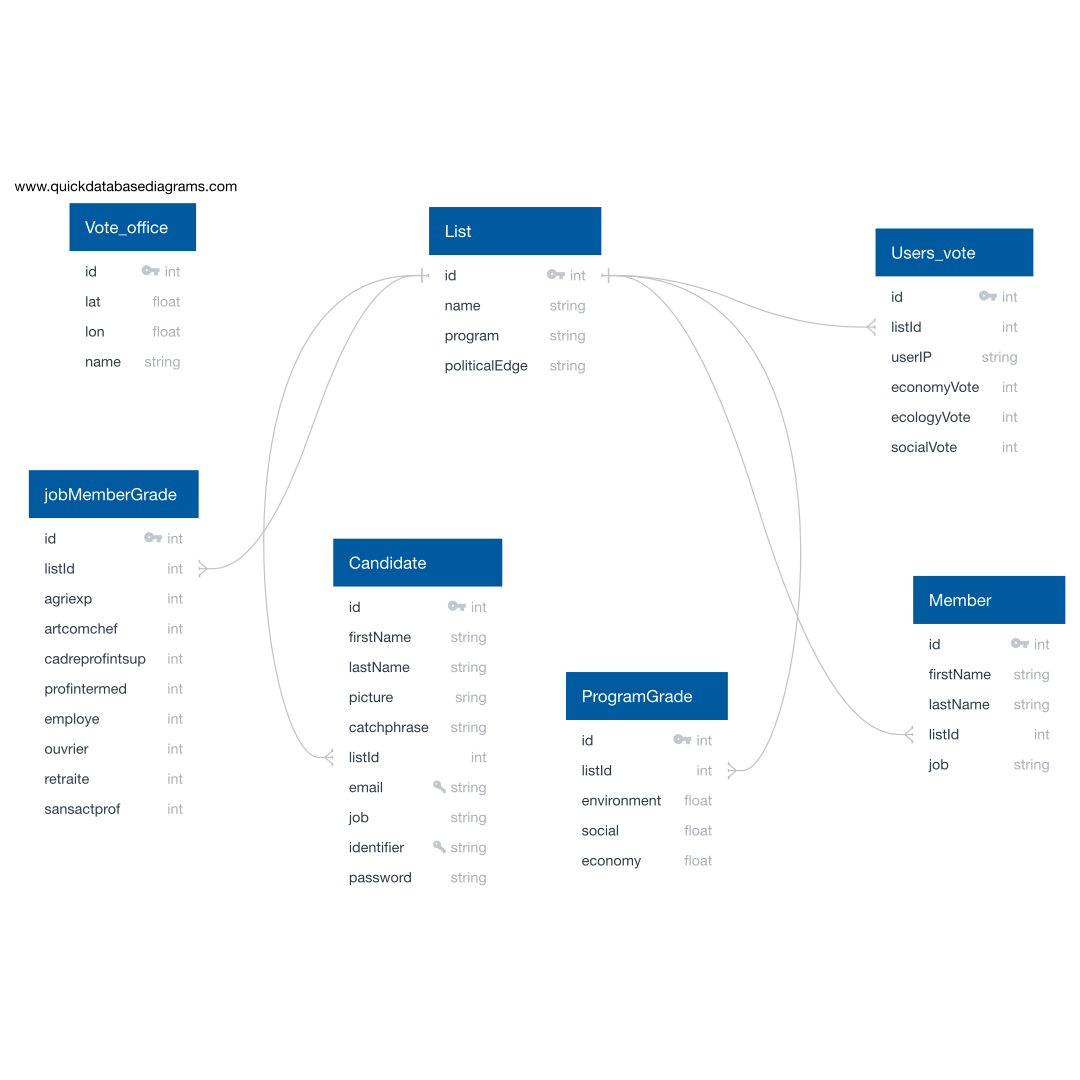
\includegraphics[scale = 0.4]{schemaBD_PPII.png}
    \caption{Schema de la base de donnée}
    \label{fig:schemaBD}
\end{figure}
\newpage

\subsubsection{Implémentation de la base de données}
\vskip 0.25cm
\noindent
Nous avons utilisé le module pysqlite3 afin d'accéder à la base de données directement dans nos fonctions de traitement des données. Quelques fonctions sont dédiées à la manipulation des données directement dans les tables comme \textit{alterDatabase.py} et permettent ainsi de faciliter l'ajout des différents candidats et de leurs identifiants de connexion.
\vskip 0.25cm
\subsection{Serveur Web}
\subsubsection{Général}
\vskip 0.25cm
\noindent
Le site est composé de 4 pages web accessibles par tous les visiteurs et possède 2 pages web accessibles par les utilisateurs qui possèdent un identifiant : les candidats.
\vskip 0.25cm
\noindent
Toutes les pages possèdent la même barre de navigation et le même pied de page. La barre de navigation diffère selon l'utilisateur et affiche uniquement les pages accessibles par ceux-ci. Le pied de page possède un lien vers chaque réseaux sociaux spécifiques à la page et un lien vers la page de Télécom Nancy. Le style des pages est géré par un layout et majoritairement du Bootstrap 5 pour quelques modifications en CSS.
\vskip 0.25cm
\subsubsection{Page d'accueil}
\vskip 0.25cm
\noindent
Le visiteur est accueilli par cette page sur le site et peut accéder à deux sections :
\begin{itemize}
    \item Comment ça marche ?
    \item Liste des candidats
\end{itemize}
\vskip 0.25cm
\noindent
Les routes menant à cette page sont \textit{'/'} et \textit{'/home'} (la route \textit{'/home'} est utilisée lorsqu'on clique sur le premier onglet dans la barre de navigation).
\vskip 0.25cm
\noindent
La première section explique le fonctionnement du site et est affichée en priorité à chaque visite de cette page. La deuxième section est à l'origine cachée et affiche la liste des candidats sous forme de cartes en fonction de leur parti politique dans les listes déroulantes correspondantes. L'affichage de ces deux sections est régulé en JavaScript afin de n'afficher qu'une seule section à la fois.
\vskip 0.25cm
\subsubsection{Carte des bureaux de vote}
\vskip 0.25cm
\noindent
Cette page affiche une carte et un itinéraire vers le bureau de vote le plus proche de l'utilisateur (les bureaux de vote sont répertoriés dans la base de données). Elle est accessible par la route \textit{'/map'}. L'utilisateur a le choix de trois moyens de transport : vélo, voiture et marche. L'API pour la carte et l'itinéraire est "mapbox" et permet donc d'avoir cette fonctionnalité de meilleur itinéraire.
\vskip 0.25cm
\subsubsection{Programme d'un candidat}
\vskip 0.25cm
\noindent
Chaque candidat possède une page plus grande que les petites cartes présentes sur la page d'accueil afin d'y afficher notamment son programme dans son intégralité, les membres de sa liste électorale et leur catégorie socio-professionnelle. Cette page est accessible grâce à la route \textit{'/program/(Prénom)/(Nom)/(Id dans la base de données)'} ce qui permet un affichage de la page spécifique à chaque candidat.
\vskip 0.25cm
\noindent
Cette page contient la fonctionnalité principale du site qui est de "noter" les programmes de chaque candidat en influant sur le pourcentage d'attention apporté aux thèmes principaux (Environnement, Social, Économie).
\vskip 0.25cm
\subsubsection{Connexion}
\vskip 0.25cm
\noindent
La page de connexion permet aux candidats d'accéder aux pages qui leur sont spécifiques pour pouvoir référencer leur programme, leur liste électorale et ajouter différentes informations pour compléter leur profil. Elle est accessible grâce à la route \textit{'/login'}. Seuls les candidats ont accès à des identifiants attribués par un gérant du site.
\vskip 0.25cm
\subsubsection{Profil de l'utilisateur}
\vskip 0.25cm
\noindent
Le profil est accessible uniquement lorsque l'on est connecté sur le site et la route suit le même principe que la route pour la page du programme d'un candidat \textit{'/profile/(Prénom)/(Nom)/(Id dans la base de données)'}. On peut y rentrer une citation et y mettre une photo de profil.
\vskip 0.25cm
\subsubsection{Référencement du programme}
\vskip 0.25cm
\noindent
Les candidats ont accès à une page afin d'y renseigner leur programme et les membres de leur liste électorale avec leur catégorie socio-professionnelle. La route d'accès pour cette page est \textit{'/defineProgram'}. La page est donc divisée en deux sections et affichent les membres déjà renseignés et le programme s'il est déjà écrit afin de le modifier à souhait.
\vskip 0.25cm
\subsection{Algorithmes de traitement}
\vskip 0.25cm
\subsubsection{Introduction}
\vskip 0.25cm
\noindent
Les algorithmes implémentés ont permis de faciliter la récupération et le traitement des données acquises via des requêtes dans la base de données afin de les réinjecter dans les pages HTML par la suite. Certains agorithmes s'occupent simplement de séparer des données, mais d'autres permettent d'introduire de nouvelles données dans (\textit{database.db}) en vue d'être utilisées ensuite sur une page web comme les statistiques par thème de chaque candidat.
\vskip 0.25cm
\subsubsection{Localisation de l'utilisateur et du bureau de vote le plus proche}
\vskip 0.25cm
\noindent
En utilisant l'API "mapbox" et une localisation à partir de l'adresse ip, nous avons réalisé des algorithmes permettant de localiser l'utilisateur, le bureau de vote le plus proche de lui, ainsi que l'itinéraire le plus rapide pour y accéder. C'est algorithmes se trouvent dans le fichier \textit{coreLocalisation.py}. 
\vskip 0.25
\subsubsection{Analyse des listes candidates}
\vskip 0.25cm
\noindent
Nous avons réaliser un algorithme qui nous permet, en récupérant les membres d'une liste et leur profession dans la base de données, insérer dans cette dernière le pourcentage de membre appartenant à chaque catégorie professionnelle. Cet algorithme est implémenté dans la fonction \textit{rateList()}, située dans le fichier \textit{memberAnalysis.py}
\vskip 0.25cm
\subsubsection{Analyse du programme d'un candidat}
\vskip 0.25cm
\noindent
Après le référencement du programme d'un candidat, celui-ci est analysé selon différents thèmes. On obtient une note sous forme de pourcentage sur ces trois thèmes. Les fonctions \textit{countWordFrequency()} et \textit{rateDataWords()} permettent de compter le nombres de mots clés liés à chaque thème dans le programme, et d'obtenir la note correspondante. Elles sont situées dans le fichier \textit{programAnalysis.py}.
